\documentclass{standalone}
\usepackage{standalone}

\begin{document}
	\section{Performance of Enhanced BWT FM-index }
	Enhanced FM-index would work very fast if a long K-mer is found. In fact, this could make more efficient excluding the rest of the computation if a very long or reliable K-mer is found. Figure \ref{fig:fmComp} shows that comparatively data with less error works more efficiently in respect to time. Below is one of the result summary snippet generated by the program.
\begin{figure}
	\centering
	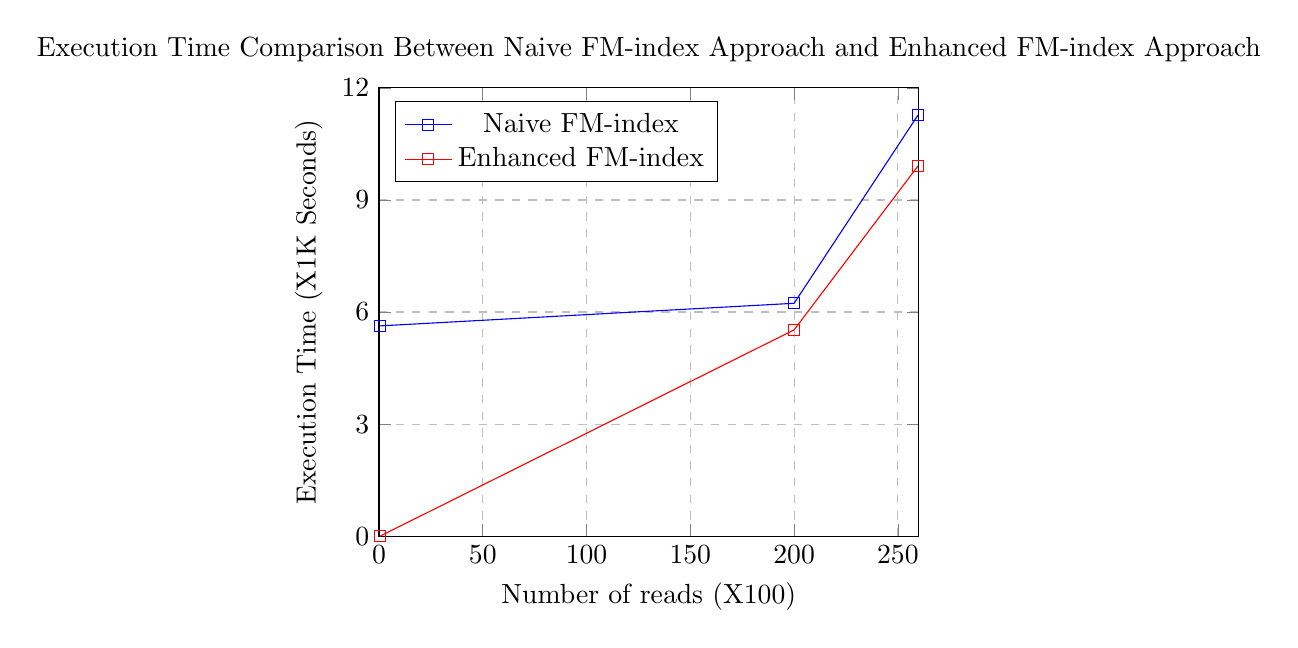
\begin{tikzpicture}
	\begin{axis}[
	title={Execution Time Comparison Between Naive FM-index Approach and Enhanced FM-index Approach},
	xlabel={Number of reads (X100)},
	ylabel={Execution Time (X1K Seconds) },
	xmin=0, xmax=260,
	ymin=0, ymax=12,
	xtick={0,50,100,150,200,250},
	ytick={0,3,6,9,12},
	legend pos=north west,
	ymajorgrids=true,
	xmajorgrids=true,
	grid style=dashed,
	]
	
	\addplot[
	color=blue,
	mark=square,
	]
	coordinates {
		( 0.50 , 5.629 )(200, 6.234)(259.70, 11.271)
	};
	\addlegendentry{Naive FM-index}
	\addplot[
	color=red,
	mark=square,
	]
	coordinates {
		(0.50 , 0.001167 )(200.00, 5.522)(259.70, 9.910)
	};
	\addlegendentry{Enhanced FM-index}
	\end{axis}
	\end{tikzpicture}
	
	
	\caption{For error free data, enhanced FM-index working very fast than naive FM-index. For noisy data, the time gap is reducing.} \label{fig:fmComp}
\end{figure}
\subsubsection*{Result Summary}
\begin{verbatim}
	 >>> INDEX CREATING <<<
	 Indexing of Reverse Reference:
	 Length of Reference: 493290
	 Reference Indexing Time: 0.177091
	 Memory Consumption in MB:
	 Forward = 0.124944
	 Reverse = 0.124959
	 
	 Indexing of Reference:
	 Length of Reference: 493290
	 Reference Indexing Time: 0.173042
	 Memory Consumption in MB:
	 Forward = 0.124951
	 Reverse = 0.124936
	 >>> END - INDEX CREATING <<<
	 Total Reads = 50
	 LOCATIONS querying Time in normal procedure: 5628.92
	 LOCATIONS querying Time in modified procedure: 1.1666
\end{verbatim}
\subsubsection*{Data Interpretation}
\begin{itemize}
	\item The length of the reference is 0.5M.
	\item Indexing time of the reference for naive FM-index is 0.17 seconds.
	\item Indexing time of the reverse reference for the enhanced FM-index is 0.18 seconds.
	\item For every type of indexing there needs to create two index, one is the main genome and other is the reverse complement of it. Each type of indexing taking 0.125 MB memory.
	\item Total Read Count is 50.
	\item Naive FM-index took 5628.92 seconds to process all of the reads.
	\item Enhanced FM-index took only 1.17 seconds to process all of the reads.
	\item For enhanced FM-index, we need to index the reference reversely. From the above report, it is clear that this does not makes any difference with respect to memory and time.
\end{itemize}
\subsubsection*{Indexing Reference}
Both of the indexes of the reference take same resources with respect to time and memory. However, The memory consumption by the index is lower in these approach comparing with the most recent tool minimap\cite{minimap}. Figure \ref{fig:fmMemIndex} shows that minimiap takes at least six times memory comparing to the both type of indexing.
\begin{figure}
	\centering
	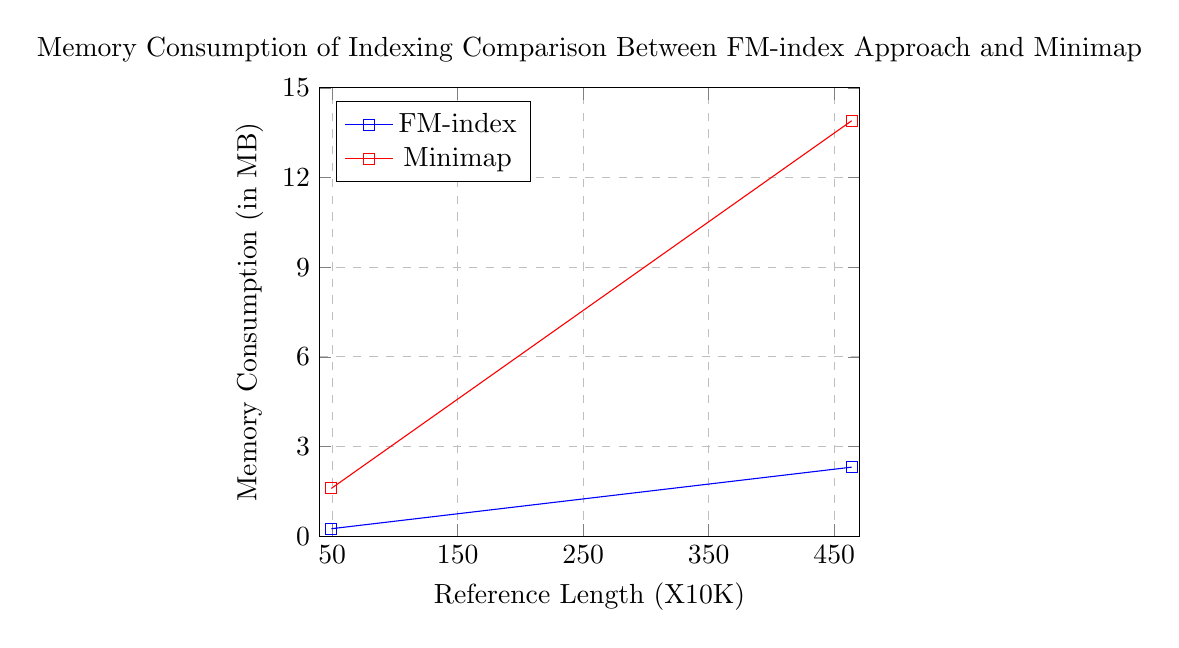
\begin{tikzpicture}
	\begin{axis}[
	title={Memory Consumption of Indexing Comparison Between FM-index Approach and Minimap},
	xlabel={Reference Length (X10K)},
	ylabel={Memory Consumption (in MB) },
	xmin=40, xmax=470,
	ymin=0, ymax=15,
	xtick={50,150,250,350,450},
	ytick={0,3,6,9,12,15},
	legend pos=north west,
	ymajorgrids=true,
	xmajorgrids=true,
	grid style=dashed,
	]
	
	\addplot[
	color=blue,
	mark=square,
	]
	coordinates {
		(49.33 , 0.25 )(463.92, 2.31)
	};
	\addlegendentry{FM-index}
	\addplot[
	color=red,
	mark=square,
	]
	coordinates {
		(49.33 , 1.6 )(463.92, 13.9)
	};
	\addlegendentry{Minimap}
	\end{axis}
	\end{tikzpicture}
	
	
	\caption{Reference Indexing Memory Consumption Comparison between FM-index Approach and Minimap.} \label{fig:fmMemIndex}
\end{figure}

\end{document}